\documentclass{cekarticle}
\usepackage{color}
\usepackage{amsmath}
\usepackage{amssymb}
\usepackage{array}

\begin{document}

%=============================================================================
% Title page
%=============================================================================

\title{Systems Biology Markup Language (SBML) Level 3 Proposal: Model Composition Features}

\author{Andrew Finney}

\authoremail{
\begin{minipage}{\textwidth}\centering
afinney@cds.caltech.edu
\end{minipage}}

\maketitlepage

%=============================================================================
\section{Introduction}
\label{sec:introduction}
%=============================================================================

This document describes proposed features for inclusion in
Systems Biology Markup Language (SBML) Level 3. This document
describes features enabling the composition of models from multiple instances of submodels.  

This document is not a definition of SBML Level 3 or part of it.
This document simply presents various features which could be
incorporated into SBML Level 3 as the Systems Biology community
wishes.  This document is intended for detailed review by that
community and to provoke alternative proposals.  
This proposal is designed to provide an alternative permutation of ideas
proposed by Martin Ginkel~\citep{ginkel:2002} and Jonathan Webb~\citep{webb:2003}.
This proposal is designed with a proposal for arrays~\citep{finney:2003} in mind
and is one important motivations for the creation of this proposal.

Throughout this
document issues that the author believes will require further
discussion have been highlighted.

For brevity the text of this document is with reference to SBML
Level 2~\citep{finney:2002f} i.e. features are described in terms
of changes to SBML Level 2.  In addition for brevity the UML diagrams in this proposal
show only new attributes and types for SBML Level 3.  For SBML Level 2 types Level 2
attributes are meant to be present in SBML Level 3.

All types proposed in this document will be derived from the
\texttt{SBase} type.


\section{Acknowledgements}

This proposal is based upon the prior proposals made by Martin Ginkel~\citep{ginkel:2002} and Jonathan Webb~\citep{webb:2003}.
This proposal has benefitted from discussions the author had with Martin and Jonathan.

\section{Overview}

A UML diagram for the proposal is shown in figure~\ref{fig:model-composition-uml}.

\begin{figure}[h]
  \vspace*{8pt}
  \centering
  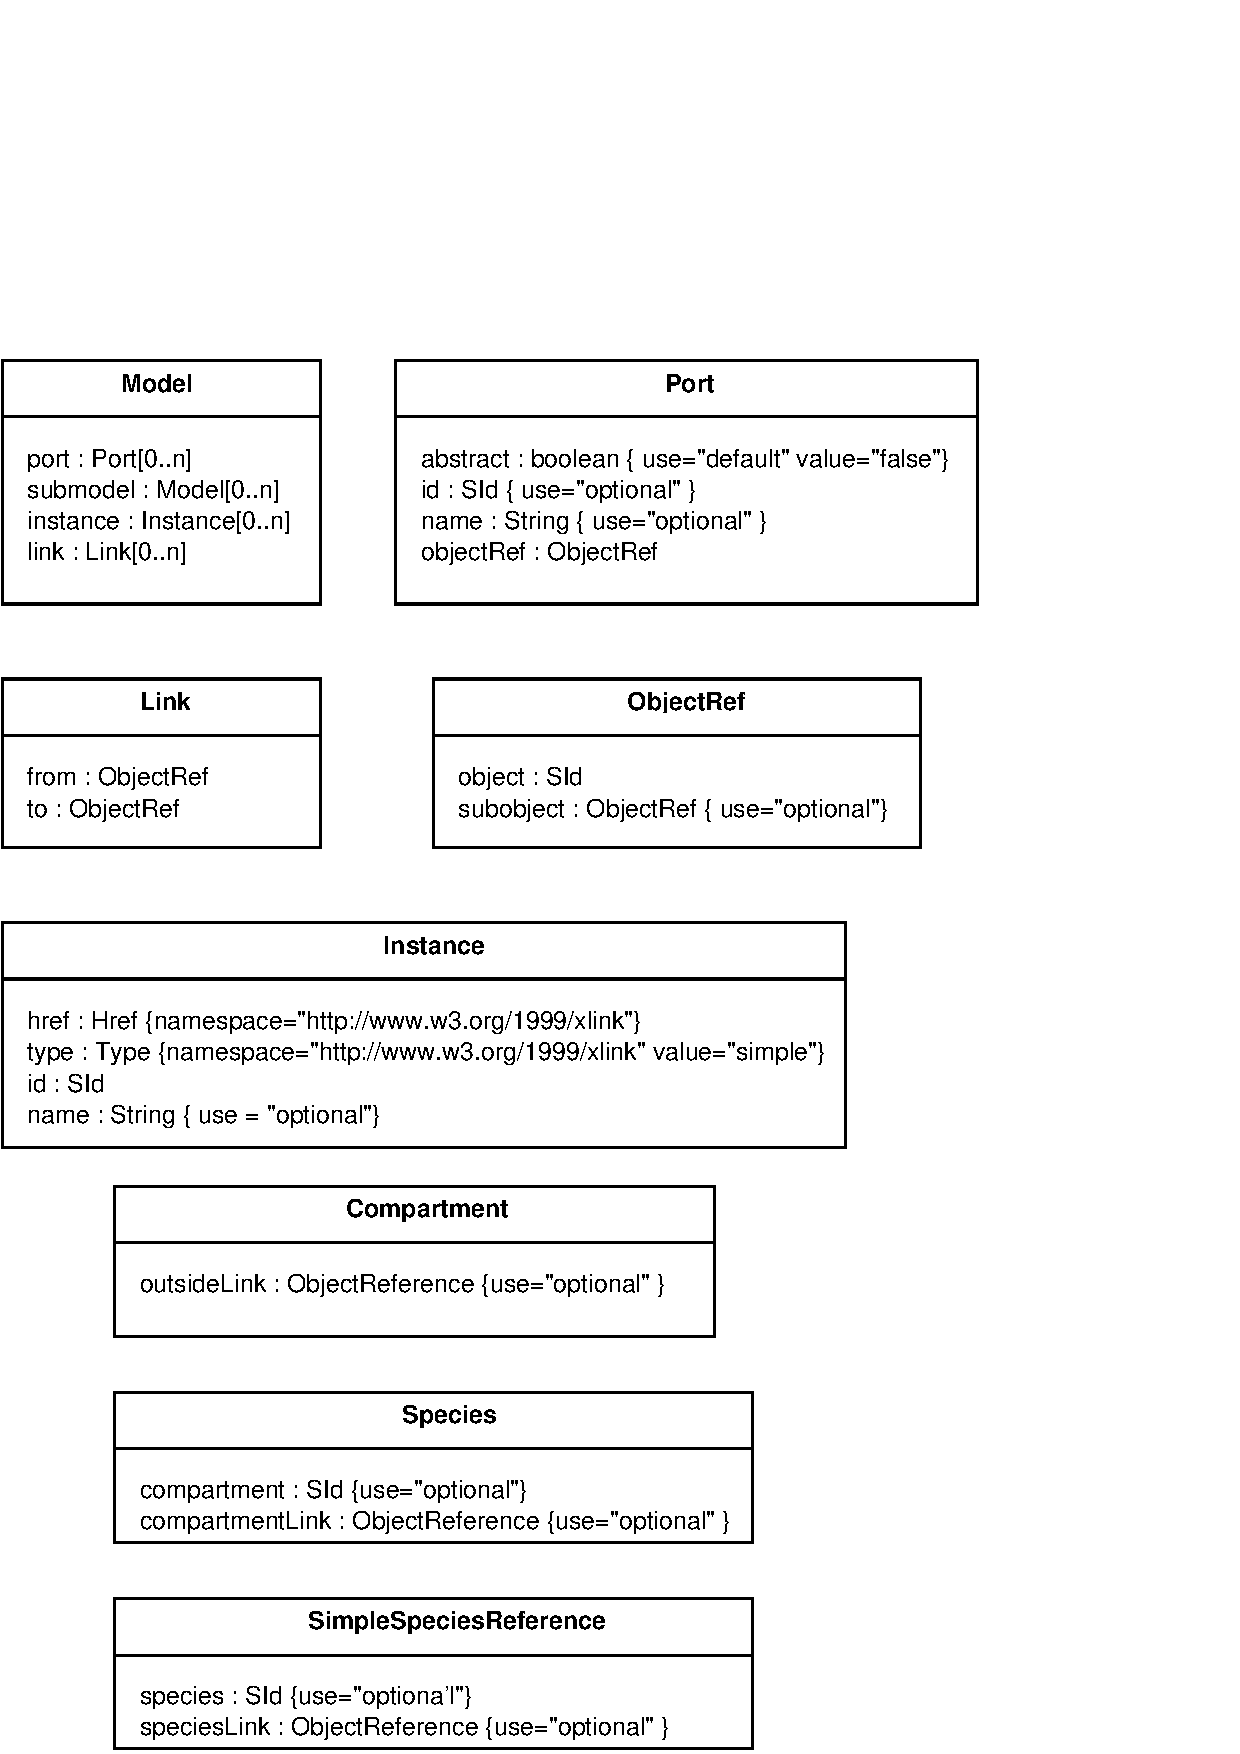
\includegraphics[scale = 0.7]{model-composition-uml}
  \caption{The types and attributes introduced into SBML by this proposal}
  \label{fig:model-composition-uml}
\end{figure}

A under this proposal a \class{Model} structure would have an optional lists of
\class{Model} (see section~\ref{sec:submodels}),
\class{Instance} (see section~\ref{sec:instances}),
\class{Link} (see section~\ref{sec:links})
and \class{Port} (see section~\ref{sec:ports}) structures.
Section~\ref{sec:objectreferences} describes the
generic mechanism for referring to objects in models that is used in this
proposal.
Complete examples of models using these proposed structures is given in section~\ref{sec:linkexamples}.

The new structures attached to \class{Model} structures are sufficient for model composition however section~\ref{sec:directlinks}
describes modifications to existing SBML Level 2 components like \class{SimpleSpeciesReference}
which enables this proposal to be more flexible.  An example is given in section~\ref{sec:egdirectlinks} which
demonstrates this feature.

\section{Submodels}
\label{sec:submodels}

In this proposal a model can contain any number of submodels.  A submodel is a full
fledged model with its own namespace: object identifiers are only in scope within the
immediate enclosing \class{Model} structure. These submodels may or may not be part
of the actual model description i.e. instances of these submodels may or may not
occur in the enclosing model.  Instances of these submodels are created through the
use of \class{Instance} structures (see section~\ref{sec:instances}). A submodel does
not have to be included within a composed model.  A submodel can be external to the
composed model (see section~\ref{sec:instances}). 

The following example shows a submodel enclosed in another model.  The submodel \texttt{inner} is redundant as no instance
of it exists in the \texttt{outer} model.

\pagebreak

\begin{example}
<?xml version="1.0"?>
<sbml xmlns="http://www.sbml.org/sbml/level3" version="1" level="3">
    <model id="outer">
        <listOfCompartments>
            <compartment id="compartmentOne" volume="1"/>
        </listOfCompartments>
        <listOfSpecies>
            <species id="S1" initialAmount="10" compartment="compartmentOne">
            <species id="X0" initialAmount="0" compartment="compartmentOne">
        </listOfSpecies>
        <listOfReactions>
            <reaction id="reaction_1" reversible="false">
                <listOfReactants>
                    <speciesReference species="X0" stoichiometry="1"/>
                </listOfReactants>
                <listOfProducts>
                    <speciesReference species="S1" stoichiometry="1"/>
                </listOfProducts>
                <kineticLaw>
                    <math xmlns="http://www.w3.org/1998/Math/MathML">
                        <apply>
                            <times/>
                            <ci> k3 </ci>
                            <ci> S1 </ci>
                        </apply>
                    </math>
                    <listOfParameters>
                        <parameter id="k3" value="0"/>
                    </listOfParameters>
                </kineticLaw>
            </reaction>
        </listOfReactions>
        <listOfSubmodels>
            <model id="inner">
                <listOfCompartments>
                    <compartment id="compartmentOne" volume="1"/>
                </listOfCompartments>
                <listOfSpecies>
                    <species id="S1" initialAmount="0" compartment="compartmentOne">
                    <species id="X0" initialAmount="0" compartment="compartmentOne">
                </listOfSpecies>
                <listOfReactions>
                    <reaction id="reaction_1" reversible="false">
                        <listOfReactants>
                            <speciesReference species="X0" stoichiometry="1"/>
                        </listOfReactants>
                        <listOfProducts>
                            <speciesReference species="S1" stoichiometry="1"/>
                        </listOfProducts>
                    </reaction>
               </listOfReactions>
            </model>
        </listOfSubModels>
    </model>
</sbml>

\end{example}

\subsection{Libraries of models}

A SBML stream can be interpreted as a library of models if the top level \texttt{Model} structure only contains a list of submodels.  The previous
example would not be considered a library.

\section{Instances}
\label{sec:instances}

Under this proposal a model can be composed of instances of submodels through the use
of \class{Instance} structures.  An \class{Instance} structure refers to a
\class{Model} structure.  An \class{Instance} structure simply represents a copy of
that \class{Model} structure within the current model.

An \texttt{Instance} structure uses XLink~\citep{derose:2001} attributes to refer to
a submodel inside or outside the stream containing the \class{Instance} structure.
The \attrib{href} attribute contains an XPointer~\citep{derose:2002} string that
points to either an SBML model document or to an model element.  If the pointer
refers to an SBML document then the pointer is equivalent to a pointer referring to
the top-level model in that document. The \attrib{type}, which must have the value
\texttt{simple}, simply indicates the XLink type of \class{Instance}. The
\texttt{Instance} structure has an \attrib{id} attribute to identify the instance.
This identifier exists in the immediate enclosing model's namespace. 

For example the following fragment, if inserted into the previous example, refers to the inner model:
\begin{example}
<listOfInstances>
    <instance
        id="innerA"
        xlink:type="simple"
        xlink:href="#xpointer(/sbml/model/listOfSubmodels/model[@id=\%22inner\%22])"/>
</listOfInstances>
\end{example}

The following fragment is an equivalent reference from another model to the original example contained in a file \texttt{X.xml}:

\begin{example}
<listOfInstances>
    <instance
        id="innerA" 
        xlink:type="simple"
        xlink:href="X.xml#xpointer(/sbml/model/listOfSubmodels/model[@id=\%22inner\%22])"/>
</listOfInstances>
\end{example}

The following fragment is a reference from another model to the top-level model contained in a file \texttt{X.xml}:

\begin{example}
<listOfInstances>
    <instance
        id="innerB"
        xlink:type="simple"
        xlink:href="X.xml"/>
</listOfInstances>
\end{example}

\subsection{Issue}

We used XLink to refer to submodels because its a standard mechanism for linking
XML elements inside and outside a given document.  XLink attributes can be interpreted
by XML aware tools.

We may wish to significantly restrict the content of the \attrib{href} attribute content to consist only of the form, in BNF

\begin{example}
   wholeURI ::= URI | XPointer
   Xpointer ::= (URI)"#xpointer(/sbml/model" modelreference* ")"
   modelReference ::= "/listOfSubmodels/model[@id=\%22" SId "\%22]" 
\end{example}

The advantage is that parsers won't be required to parse and execute the whole XPath syntax which may require SBML streams
to be stored in DOM form for access by generic XPointer evaluators.  However tools that can interpret the full XPath syntax would
still be able to interpret the XLink attributes.
This restricted form is unambiguous unlike some potential XPath strings.

\section{Object References}
\label{sec:objectreferences}

Each instance structure has an \emph{implied} content which reflects the content of the referenced \class{Model} structure.
This section describes an scheme for referencing the structures implied by instances.
This scheme is required so that links can be made between models.  These links enable a model composed of instances to be literally more
than a sum of its parts (see section~\ref{sec:links}).

The implied content of an instance doesn't correspond directly to any XML structure.  For example consider 2 instances which reference
the same submodel.  There doesn't exist anywhere the 2 XML elements that
represent the components that are implied by the 2 instances and thus it is not seem appropriate to use XML addressing schemes such as
XPointer to reference them.  Instead this section proposes a reference scheme
specific to SBML Level 3.

The \class{ObjectRef} structure is used to refer to content implied by instances.  The object referenced by a single \class{ObjectRef}
structure depends on the context and the content of the structure's \attrib{object}
field.  
The \attrib{object} field can refer to components including 
instances but not models.  
If the \class{ObjectRef} is not contained within another
\class{ObjectRef} then the \attrib{object} field refers to a component in the
immediate enclosing \class{Model} structure.  In any context if the \attrib{object}
field refers to an instance or a reaction the \class{ObjectRef} structure must
contain a \attrib{subobject} attribute i.e. a nested \class{ObjectRef}.

Consider a \class{ObjectRef} structure enclosed inside another \class{ObjectRef}
structure where the enclosing structure refers to an instance.
The enclosed structure can refer to a component in the
submodel referenced by that instance.  If this referenced component is an
instance then the process continues recursively building up a path to a component.

Consider a \class{ObjectRef} structure enclosed inside another \class{ObjectRef}
structure where the enclosing structure refers to a reaction.
The enclosed structure can refer only to parameters defined within the reaction.

This scheme deliberately cannot create references to instances, models or reactions.

In the following examples the outer \class{ObjectRef} is contained in arbitrarily
named field \attrib{test}.  All these examples are located in the top level model
of the model example above.  The first example refers to the top-level
species \texttt{S1}.

\begin{example}
<test object="S1"/>
\end{example}

The following example refers to the parameter of the reaction in the top level model

\begin{example}
<test object="reaction_1">
    <subobject object="k3"/>
</test>
\end{example}

The remaining example in this section is based on the following instance occurring in the model

\begin{example}
<listOfInstances>
    <instance
        id="innerA" 
        xlink:type="simple" 
        xlink:href="#xpointer(/sbml/model/listOfSubmodels/[@id=\%22inner\%22])"/>
</listOfInstances>
\end{example}

The following example refers to the species \texttt{S1} contained inside instance \texttt{innerA}.

\begin{example}
<test object="innerA">
    <subobject object="S1"/>
</test>
\end{example}

\subsection{Issue}

Given the form of model composition given here we could use a simpler form consisting of an attribute containing a
sequence of \class{SId} strings separated by whitespace. Such scheme would be difficult to extend to incorporate planned
Level 3 features such as arrays.

\section{Links}
\label{sec:links}

To enable models to be meaningfully composed linkages between instances need to be
created.  A model can contain a set of \class{Link} elements each of which contain 2
\class{ObjectRef}
fields: \attrib{from} and \attrib{to}.
These fields can only refer to ports, species, parameter and compartment components
in the top level model and/or 
implied within instances.

A \class{Link} structure should interpreted as follows.  The object referenced by the
\attrib{from} field (\emph{from object})
merges with the object referenced by the \attrib{to} field (\emph{to object}) to
become the same entity.  These objects are called the referenced objects. 
The attribute values 
of the \emph{to object}
are replaced by those of the \emph{from object}.
%The value of an optional attribute without a default
% (e.g. \attrib{initialAmount} on
%\class{Species}) is either taken from the referenced object on which the attribute value is
%supplied or from the \emph{from object} if it is supplied
% by both objects.
 Structures (e.g. \class{SpeciesReference}) that refer to either
object effectively refer to the combined entity.
Any assignment rules that control the value of a \emph{from object} replace those
controlling a \emph{to object}.  The merged entities should obey all the semantic rules
of SBML Level 2.

The interpretation of a \class{Link} structure referencing a port is described 
in section~\ref{sec:ports}.

In any list of links in a model an object cannot be referenced by more than one \attrib{to} field in the list.
i.e. an object can't be overloaded twice at the same level in the instance hierarchy.  However it is possible for an object
to be referenced by more than one \attrib{from} field in the list i.e. an object can overload more than one object.
An object can't be referenced from a \attrib{to} field and a \attrib{from} field in the same list.

For example given the following instance in the model above.

\begin{example}
<listOfInstances>
    <instance
        id="innerA"
        xlink:type="simple"
        xlink:href="#xpointer(/sbml/model/listOfSubmodels/model[@id=\%22inner\%22])"/>
</listOfInstances>
\end{example}

We can define a link from species \texttt{S1} in the top level model to the species \texttt{X0} in the \texttt{innerA} instance.

\begin{example}
<listOfLinks>
    <link>
        <from object="S1"/>
        <to object="innerA">
            <subobject object="X0"/>
        </to>
    </link>
</listOfLinks>
\end{example}

The concentration of the combined object is 10.  The combined object is produced by \texttt{reaction\_1} in the top level model and
consumed by \texttt{reaction\_1} in instance \texttt{innerA}.

See section~\ref{sec:eg} for a complete example.

\subsection{Link Validity}
\label{sec:linkvalidity}

It should be obvious that for a composed model to work correctly some restrictions
should be imposed on the linkages that can be made.  It is not yet clear how far this
should be defined as part of the language.  Some parts of this section could be regarded
as guidance for software that may wish to check the state of models during composition.

\subsubsection{Type correspondence}
\label{sec:typecorrespondence}

Components of different types (species, compartment or parameter) cannot
be linked.

\subsubsection{Unit Correspondence}
\label{sec:unitcorrespondence}

The unit system of SBML Levels 1 and 2 was designed with model composition in mind.
Linked components can be checked to ensure that their assigned units match. 

\section{Ports}
\label{sec:ports}

Although there is no consensus for it in the biochemical network modelling community some researchers
believe that submodels need to have well defined interfaces to successfully support model composition.
Briefly the arguments for having interfaces are as follows.
\begin{itemize}
\item An interface provides a ``contract'' between a submodel and models composed
from that submodel.  The contract can be 
maintained even when the submodel internals are significantly changed.
\item The contract can be ``implemented'' by several alternative submodels with the same interface.  These
alternative submodels may use different simulation paradigms and/or encode different hypotheses for the modelled
phenomena. 
\item The interface facilitates the documentation of the function of the submodel from the perspective of a modeller
wishing to reuse the submodel.
\end{itemize}

The counter argument is that any hierarchy in biochemical networks is only used to structure the human knowledge
of the networks.  A modeler can't anticipate all the connections that may be discovered between submodels in those
networks.  What works in software forward engineering may not work in biochemical network reverse engineering.

This proposal doesn't enforce the use of interfaces but does allow the definition of model interfaces and
the linking to/from objects on an interface.  Under this proposal it is valid to simultaneously use and ignore model interfaces.

Under this proposal a model's interface is defined by the list of \class{Port} structures contained in the model.
A \class{Port} structure has an object reference field which refers to a given component within the model (including
components inside instances).  The other fields on the \class{Port} structure are optional \attrib{id} and
\attrib{name} fields.  If the \attrib{id} attribute is not present then a \class{Port} structure simply indicates
that the referenced object is part of the defined interface.  If the \attrib{id} attribute is present then its value
can be used as alternative alias for the referenced object.  This alias is for use in object reference structures and
in other \class{SId} fields.  The alias is in the containing model's component namespace.

The \attrib{abstract} optional boolean attribute on the \class{Port} structures indicates that the referenced
object is ``designed'' to be referenced by the \attrib{to} field of a \class{Link} structure (it is an \emph{abstract port}).
The \attrib{abstract} field has only a documentation function: tools may or may not wish to raise errors when an
\emph{abstract port} is used as a \emph{from object}.

A \class{Link} structure references a port by using the port's \attrib{id} field value.
The semantics of such a link are identical to a link that references the object referenced by the port.

\section{Examples using Links}
\label{sec:linkexamples}

This section contains complete model examples using links.

\subsection{Model Composition Without Ports}
\label{sec:eg}

Figure~\ref{fig:eg} shows the important components and relationships of the following example model
\begin{figure}[h]
  \vspace*{8pt}
  \centering
  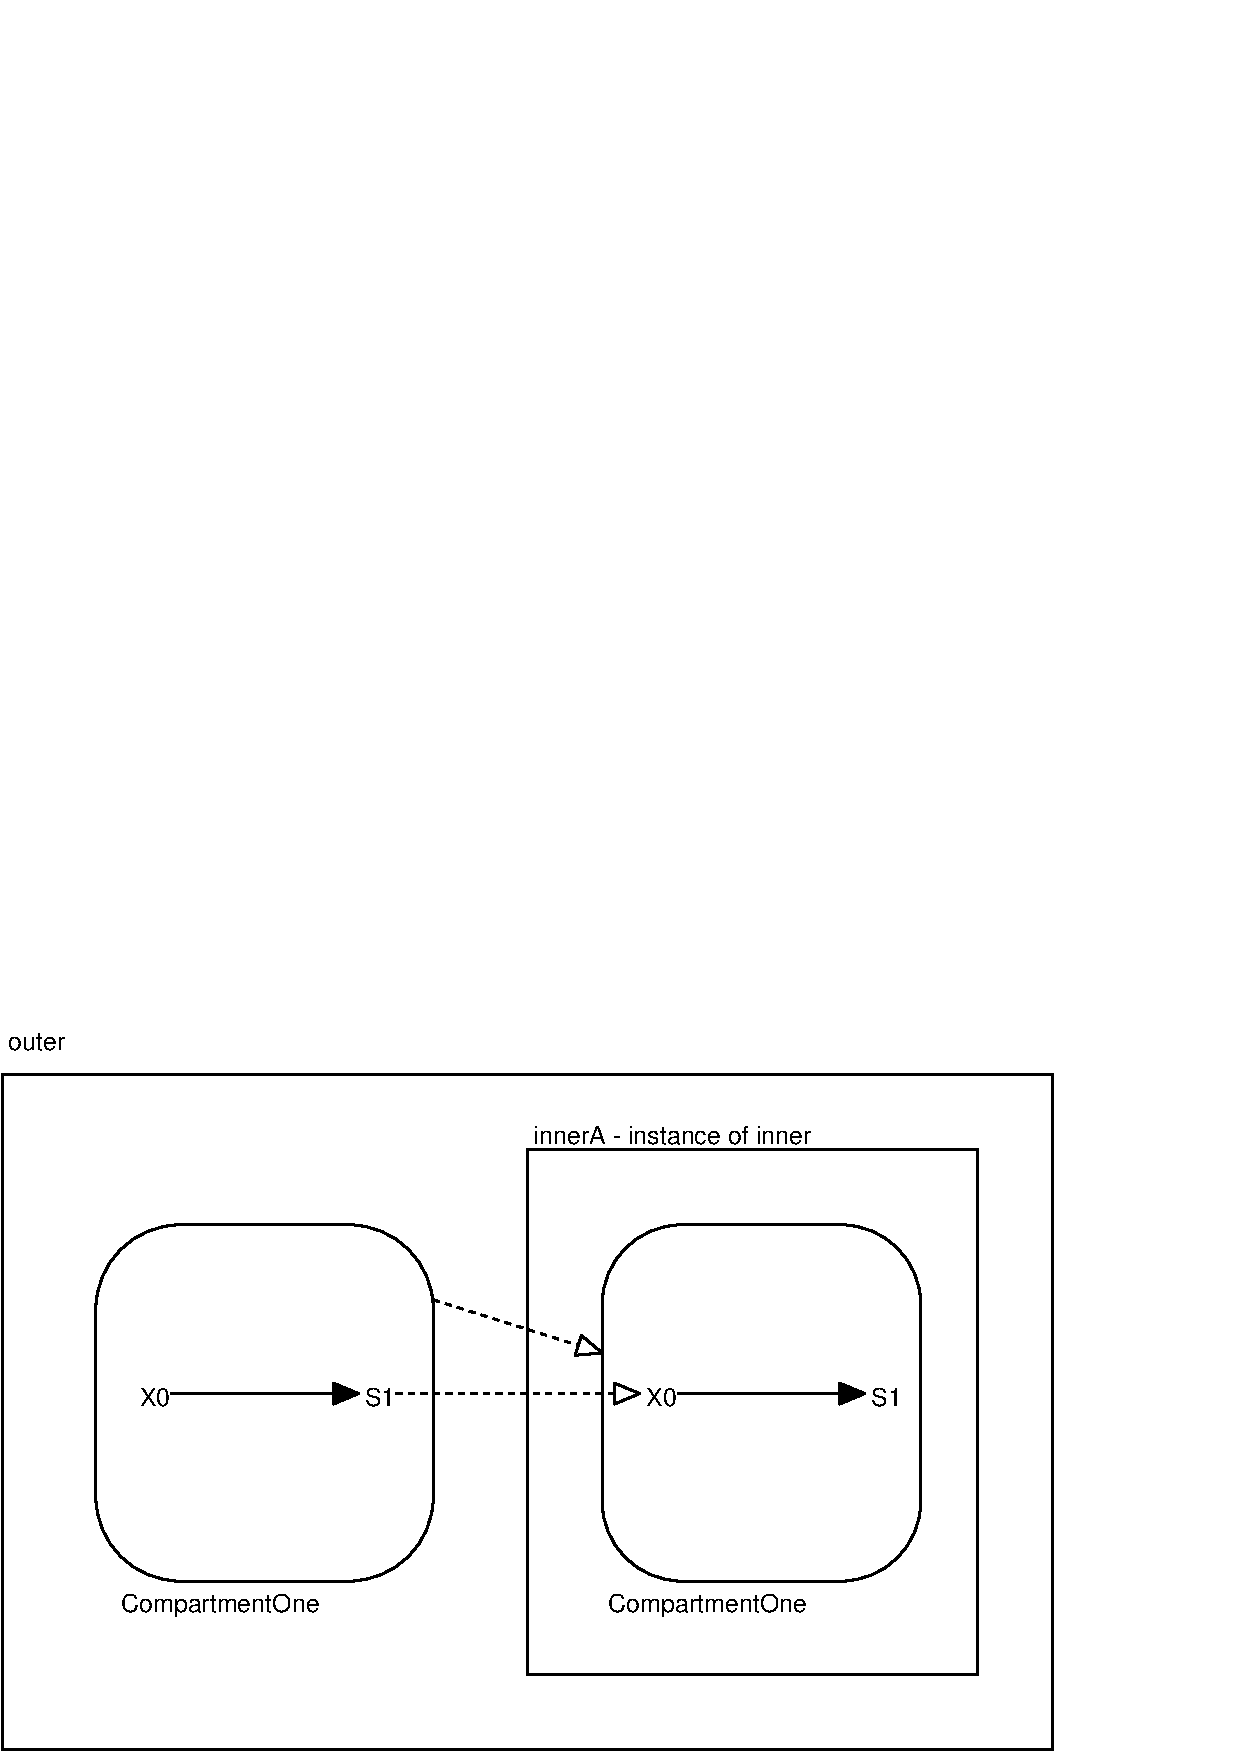
\includegraphics[scale = 0.7]{eg}
  \caption{The structure of the \texttt{outer} model.
  The rounded rectangles are compartments.
  The proper rectangles are model instances. Dashed arrows are links.
  Solid arrows are reactions.}
  \label{fig:eg}
\end{figure}

\pagebreak

\begin{example}
<?xml version="1.0"?>
<sbml xmlns="http://www.sbml.org/sbml/level3" version="1" level="3">
    <model id="outer">
        <listOfCompartments>
            <compartment id="compartmentOne" volume="1"/>
        </listOfCompartments>
        <listOfSpecies>
            <species id="S1" initialAmount="10" compartment="compartmentOne">
            <species id="X0" initialAmount="0" compartment="compartmentOne">
        </listOfSpecies>
        <listOfReactions>
            <reaction id="reaction_1" reversible="false">
                <listOfReactants>
                    <speciesReference species="X0" stoichiometry="1"/>
                </listOfReactants>
                <listOfProducts>
                    <speciesReference species="S1" stoichiometry="1"/>
                </listOfProducts>
            </reaction>
        </listOfReactions>
        <listOfSubmodels>
            <model id="inner">
                <listOfCompartments>
                    <compartment id="compartmentOne" volume="1"/>
                </listOfCompartments>
                <listOfSpecies>
                    <species id="S1" initialAmount="0" compartment="compartmentOne">
                    <species id="X0" initialAmount="0" compartment="compartmentOne">
                </listOfSpecies>
                <listOfReactions>
                    <reaction id="reaction_1" reversible="false">
                        <listOfReactants>
                            <speciesReference species="X0" stoichiometry="1"/>
                        </listOfReactants>
                        <listOfProducts>
                            <speciesReference species="S1" stoichiometry="1"/>
                        </listOfProducts>
                    </reaction>
                </listOfReactions>
            </model>
        </listOfSubModels>
        <listOfInstances>
            <instance
                id="innerA" 
                xlink:type="simple"
                xlink:href="#xpointer(/sbml/model/listOfSubmodels/model[@id=\%22inner\%22])"/>
        </listOfInstances>
        <listOfLinks>
            <link>
                <from object="S1"/>
                <to object="innerA">
                    <subobject object="X0"/>
                </to>
            </link>
            <link>
                <from object="compartmentOne"/>
                <to object="innerA">
                    <subobject object="compartmentOne"/>
                </to>
            </link>
        </listOfLinks>
    </model>
</sbml>
\end{example}

Figure~\ref{fig:eg-implied} shows the structure implied by the \texttt{outer} example model.

\begin{figure}[h]
  \vspace*{8pt}
  \centering
  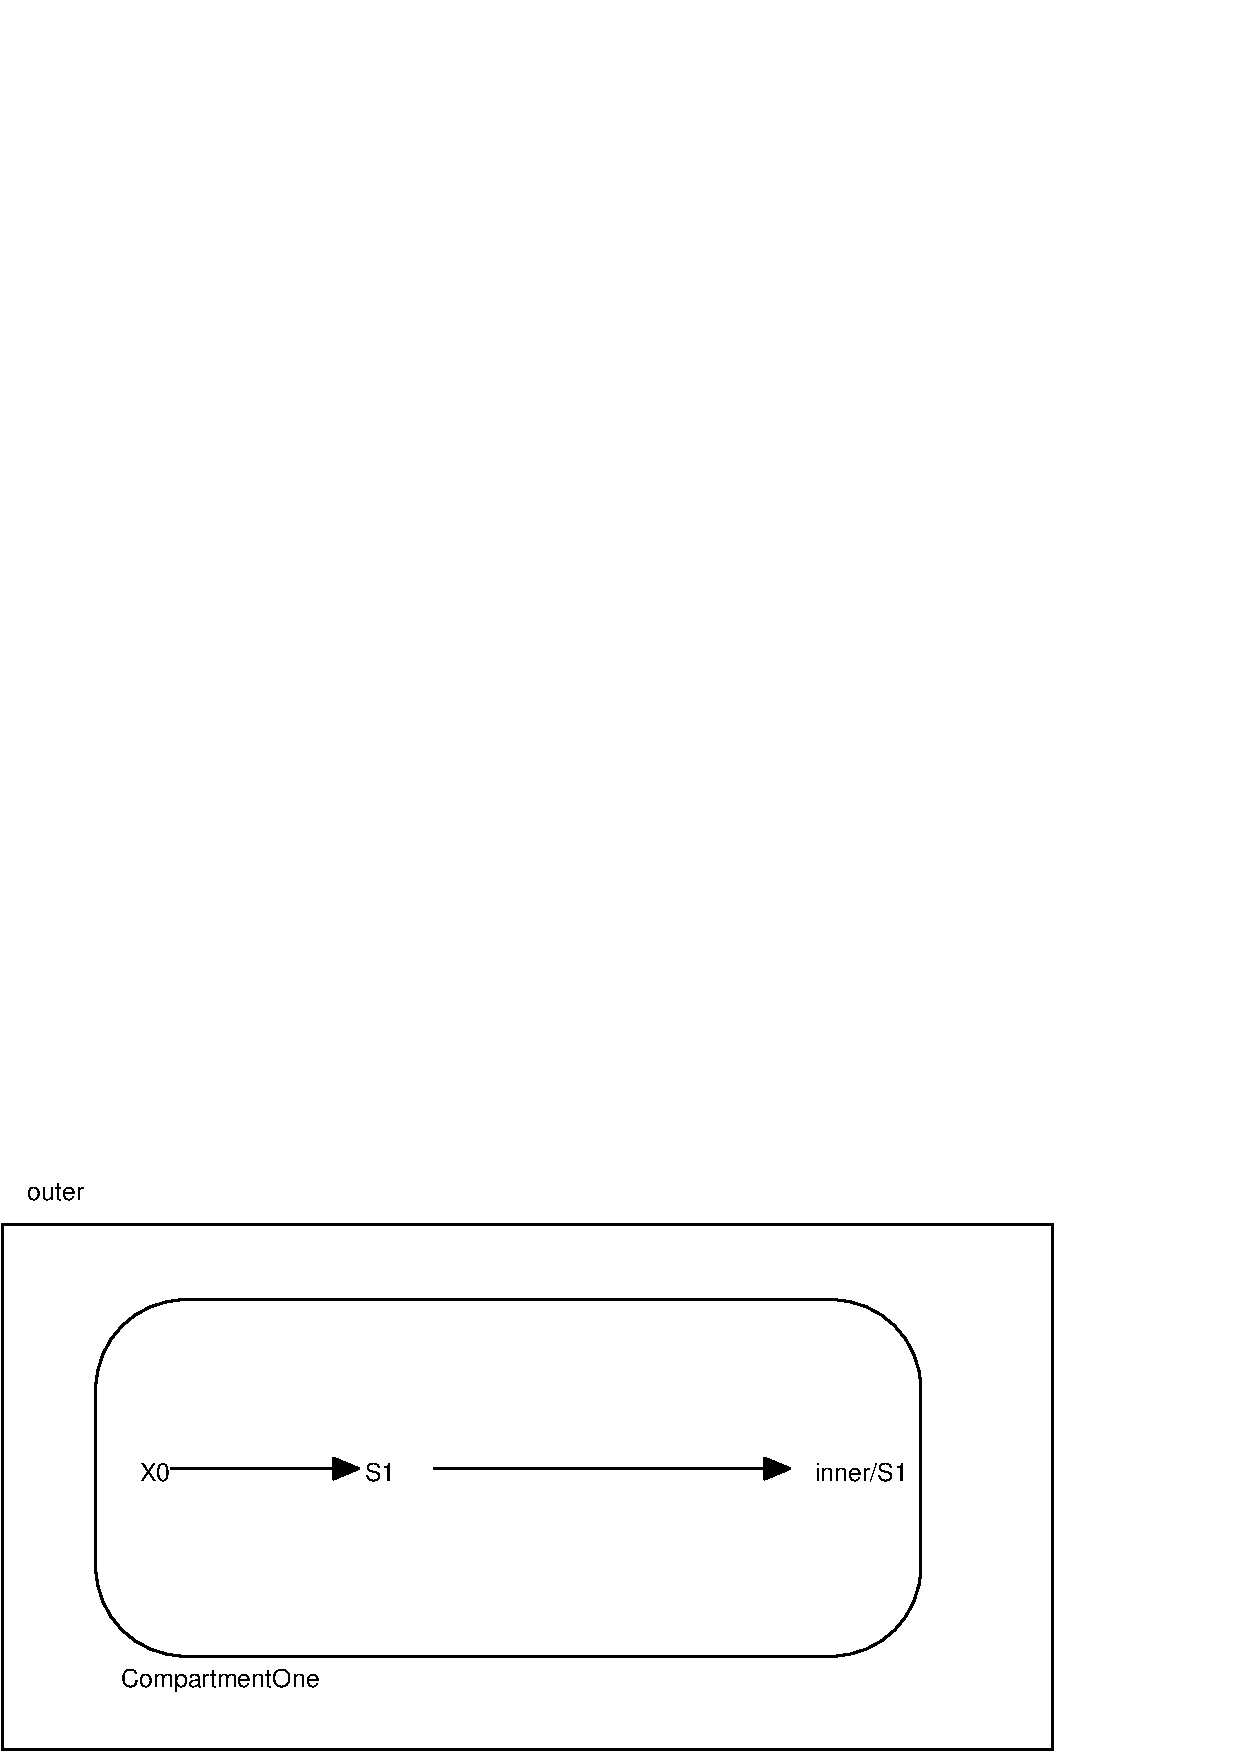
\includegraphics[scale = 0.7]{eg-implied}
  \caption{The implied form of the \texttt{outer} model}
  \label{fig:eg-implied}
\end{figure}

\subsection{Model Composition with Ports}
\label{sec:egwithports}

Figure~\ref{fig:egwithports} shows the important components and relationships of the following example model.
The implied structure of this model is the same as that shown in figure~\ref{fig:eg-implied}.
\begin{figure}[h]
  \vspace*{8pt}
  \centering
  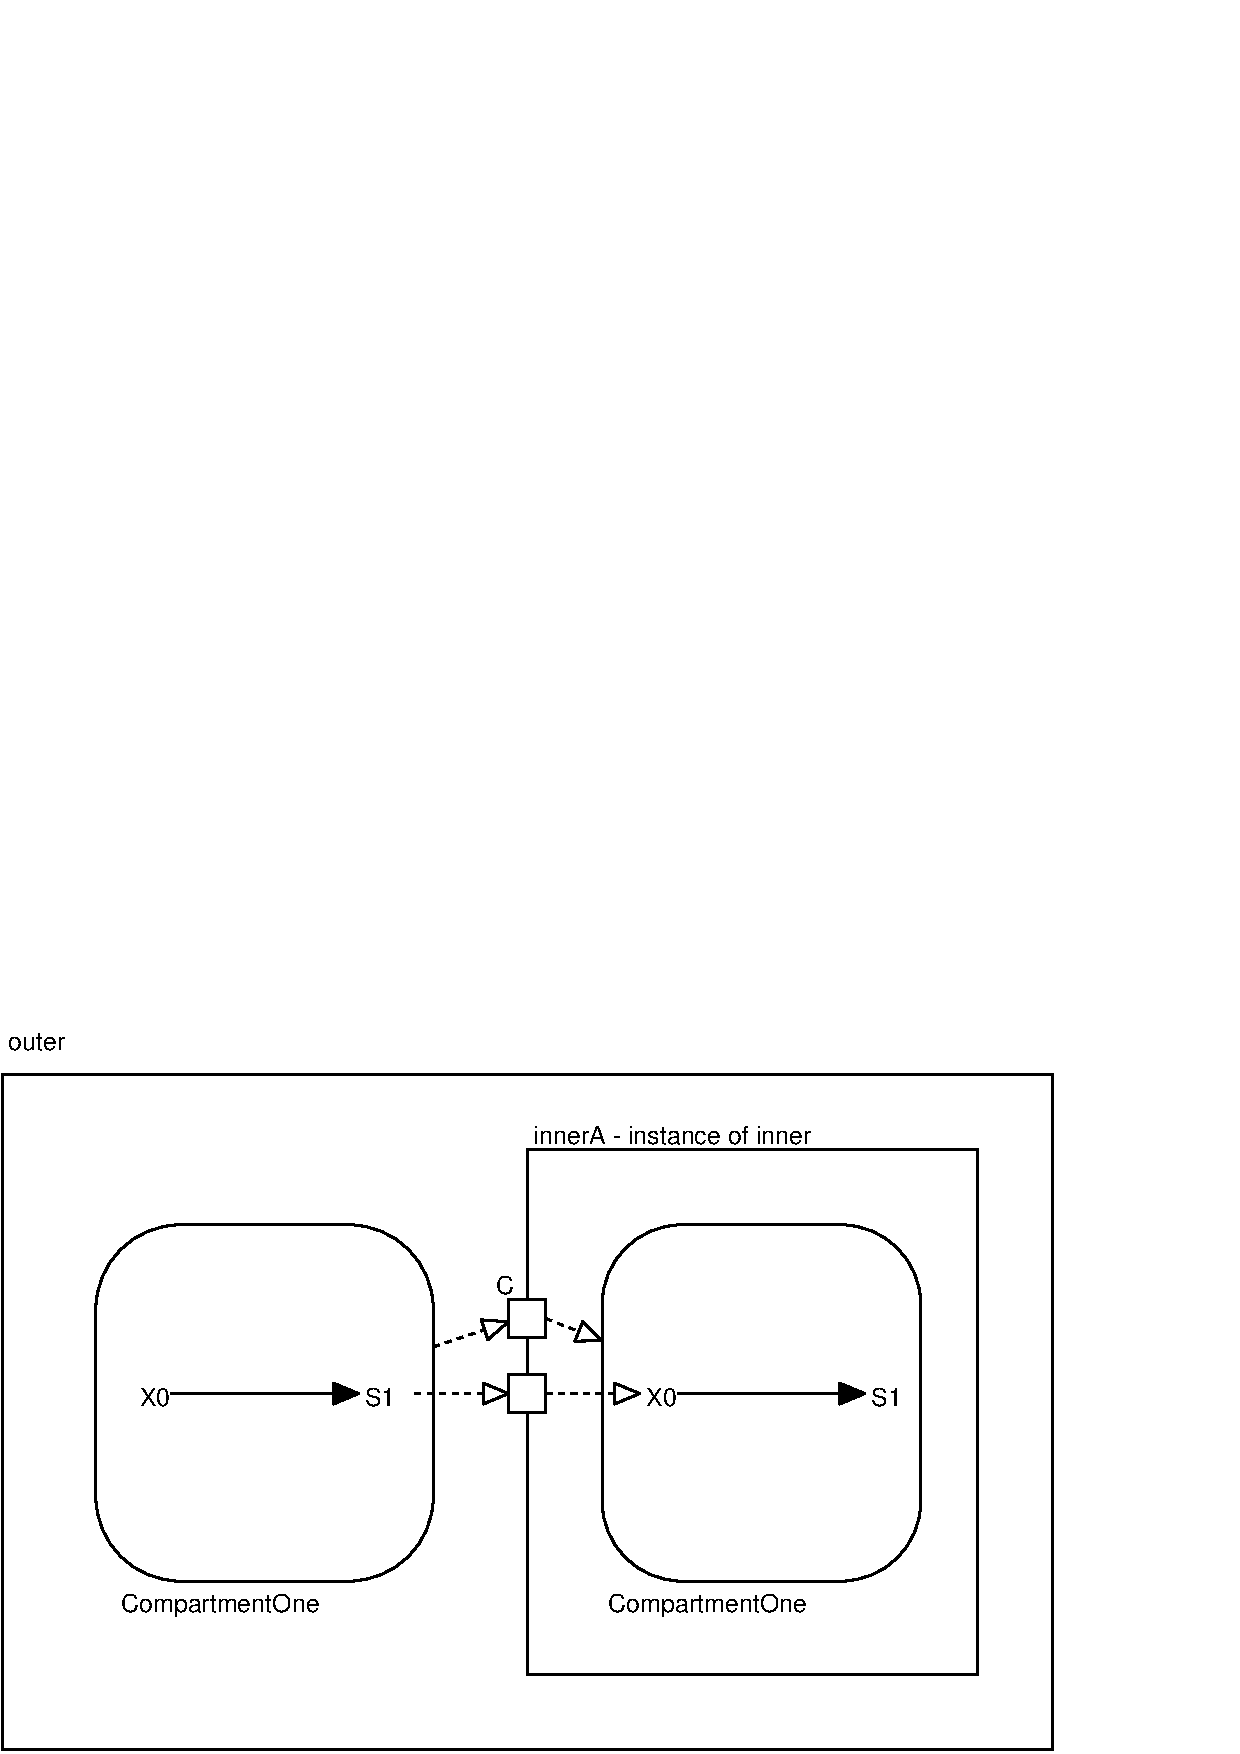
\includegraphics[scale = 0.7]{egwithports}
  \caption{The structure of the \texttt{outer\_with\_ports} model}
  \label{fig:egwithports}
\end{figure}

\begin{example}
<?xml version="1.0"?>
<sbml xmlns="http://www.sbml.org/sbml/level3" version="1" level="3">
    <model id="outer_with_ports">
        <listOfCompartments>
            <compartment id="compartmentOne" volume="1"/>
        </listOfCompartments>
        <listOfSpecies>
            <species id="S1" initialAmount="10" compartment="compartmentOne">
            <species id="X0" initialAmount="0" compartment="compartmentOne">
        </listOfSpecies>
        <listOfReactions>
            <reaction id="reaction_1" reversible="false">
                <listOfReactants>
                    <speciesReference species="X0" stoichiometry="1"/>
                </listOfReactants>
                <listOfProducts>
                    <speciesReference species="S1" stoichiometry="1"/>
                </listOfProducts>
            </reaction>
        </listOfReactions>
        <listOfSubmodels>
            <model id="inner">
                <listOfCompartments>
                    <compartment id="compartmentOne" volume="1"/>
                </listOfCompartments>
                <listOfSpecies>
                    <species id="S1" initialAmount="0" compartment="compartmentOne">
                    <species id="X0" initialAmount="0" compartment="compartmentOne">
                </listOfSpecies>
                <listOfReactions>
                    <reaction id="reaction_1" reversible="false">
                        <listOfReactants>
                            <speciesReference species="X0" stoichiometry="1"/>
                        </listOfReactants>
                        <listOfProducts>
                            <speciesReference species="S1" stoichiometry="1"/>
                        </listOfProducts>
                    </reaction>
                </listOfReactions>
                <listOfPorts>
                    <port object="X0"/>
                    <port id="C" object="compartmentOne"/>
                </listOfPorts>
            </model>
        </listOfSubModels>
        <listOfInstances>
            <instance
                id="innerA" 
                xlink:type="simple"
                xlink:href="#xpointer(/sbml/model/listOfSubmodels/model[@id=\%22inner\%22])"/>
        </listOfInstances>
        <listOfLinks>
            <link>
                <from object="S1"/>
                <to object="innerA">
                    <subobject object="X0"/>
                </to>
            </link>
            <link>
                <from object="compartmentOne"/>
                <to object="innerA">
                    <subobject object="C"/>
                </to>
            </link>
        </listOfLinks>
    </model>
</sbml>
\end{example}

%-----------------------------------------------------------------------

\section{Direct Links}
\label{sec:directlinks}

One of the problems with the proposal as described in the previous sections
is that some forms of model composition that ought to be simple are less than
straightforward.  For example consider the composition of two models together
simply by creating a reaction between them (an outer model contains two instances
and a reaction).  Using the above form we would have to create new species
for all the reaction's products, reactants and modifiers.  These species would be linked
to the appropriate species inside the instances.  A more appropriate approach
would be to enable the \class{SimpleSpeciesReference} structures of the reaction
to reference the species inside the instances directly.
This section proposed some modifications to existing structures of SBML
to facilitate this kind of direct link.

Under this proposal, as shown in figure~\ref{fig:model-composition}, types like
\class{Species} have an additional field of type 
\class{ObjectRef} which can refer to objects inside instances.  This field is an
alternative to an existing \class{SId} field.

On \class{Compartment} the \class{ObjectRef} field \attrib{outsideLink}
is an alternative to the \class{SId} field \attrib{outside}.  Similarly
on \class{Species} \attrib{compartmentLink} is an
alternative to \attrib{compartment}, on \class{SimpleSpeciesReference} \attrib{speciesLink} is
an alternative to \attrib{species} and
on \class{SingleVariableRule} \attrib{variableLink} is an alternative to the \attrib{variable}.
In each of the types one and only one of
these fields (\class{SId} or \class{ObjectRef}) can have a value.
For example \class{Species} structures can contain
a value for \attrib{compartment} or \attrib{compartmentLink} but not both.
It is not possible for both the \class{SId} or \class{ObjectRef} fields to be
omitted except in the case of the \attrib{outside} and \attrib{outsideLink} fields.

In each case the \class{ObjectRef} field
can refer to an object of the appropriate type inside any instance, for example \class{Compartment}
in the case of \attrib{compartmentLink} and \attrib{outsideLink}, \class{Species} in the case
of \attrib{speciesLink}. Section~\ref{sec:egdirectlinks} has an examples of a complete model using these fields.


The following example fragment is of a reaction transforming species \texttt{f} in instance \texttt{a} 
into species \texttt{e} in instance \texttt{b}.
\begin{example}
<reaction id="reaction_1" reversible="false">
    <listOfReactants>
        <speciesReference stoichiometry="1">
            <speciesLink object="a">
                <objectRef object="f"/>
            </speciesLink>
        </speciesReference>
    </listOfReactants>
    <listOfProducts>
        <speciesReference stoichiometry="1">
            <speciesLink object="b">
                <objectRef object="e"/>
            </speciesLink>
        </speciesReference>
    </listOfProducts>
</reaction>
\end{example}

\subsection{Direct links using ports}

These new \class{ObjectRef} fields can reference port objects of the appropriate type in which
case the direct link is equivalent to a direct link to the object referenced by the port structure.

\subsection{Direct links in math expressions}

To support direct links in math expressions we we
use a SBML specific operator via the the MathML \texttt{csymbol} element.
This SBML operator has the URI, \texttt{http://www.sbml.org/symbols/instanceselector}.
The \texttt{instanceselector} that takes an 2 arguments: the first is an instance of a submodel
the second argument is an object inside that instance.

For example we can extend the previous fragment to contain a simple kinetic law referring to the reactant.

\begin{example}
<reaction id="reaction_1" reversible="false">
    <listOfReactants>
        <speciesReference stoichiometry="1">
            <speciesLink object="a">
                <objectRef object="f"/>
            </speciesLink>
        </speciesReference>
    </listOfReactants>
    <listOfProducts>
        <speciesReference stoichiometry="1">
            <speciesLink object="b">
                <objectRef object="e"/>
            </speciesLink>
        </speciesReference>
    </listOfProducts>
    <kineticLaw>
        <math 
            <apply>
                <times/>
                <cn>0.1</cn>
                <apply>
                    <csymbol
                        encoding="SBML"
                        definitionURL="http://www.sbml.org/symbols/instanceselector">
                        .
                    </csymbol>
                    <ci>a</ci>
                    <ci>f</ci>
                </apply>
            </apply>    
        </math>
    </kienticLaw>
</reaction>
\end{example}

\section{Example of Direct links}
\label{sec:egdirectlinks}

The following model consists of two instances of a simple submodel.
The submodel contains two species with a reaction between them.
The top level model contains a reaction which links the two submodels
together.  Figure~\ref{fig:egdirectlinks} shows the important components and relationships 
of the model.
\begin{figure}[h]
  \vspace*{8pt}
  \centering
  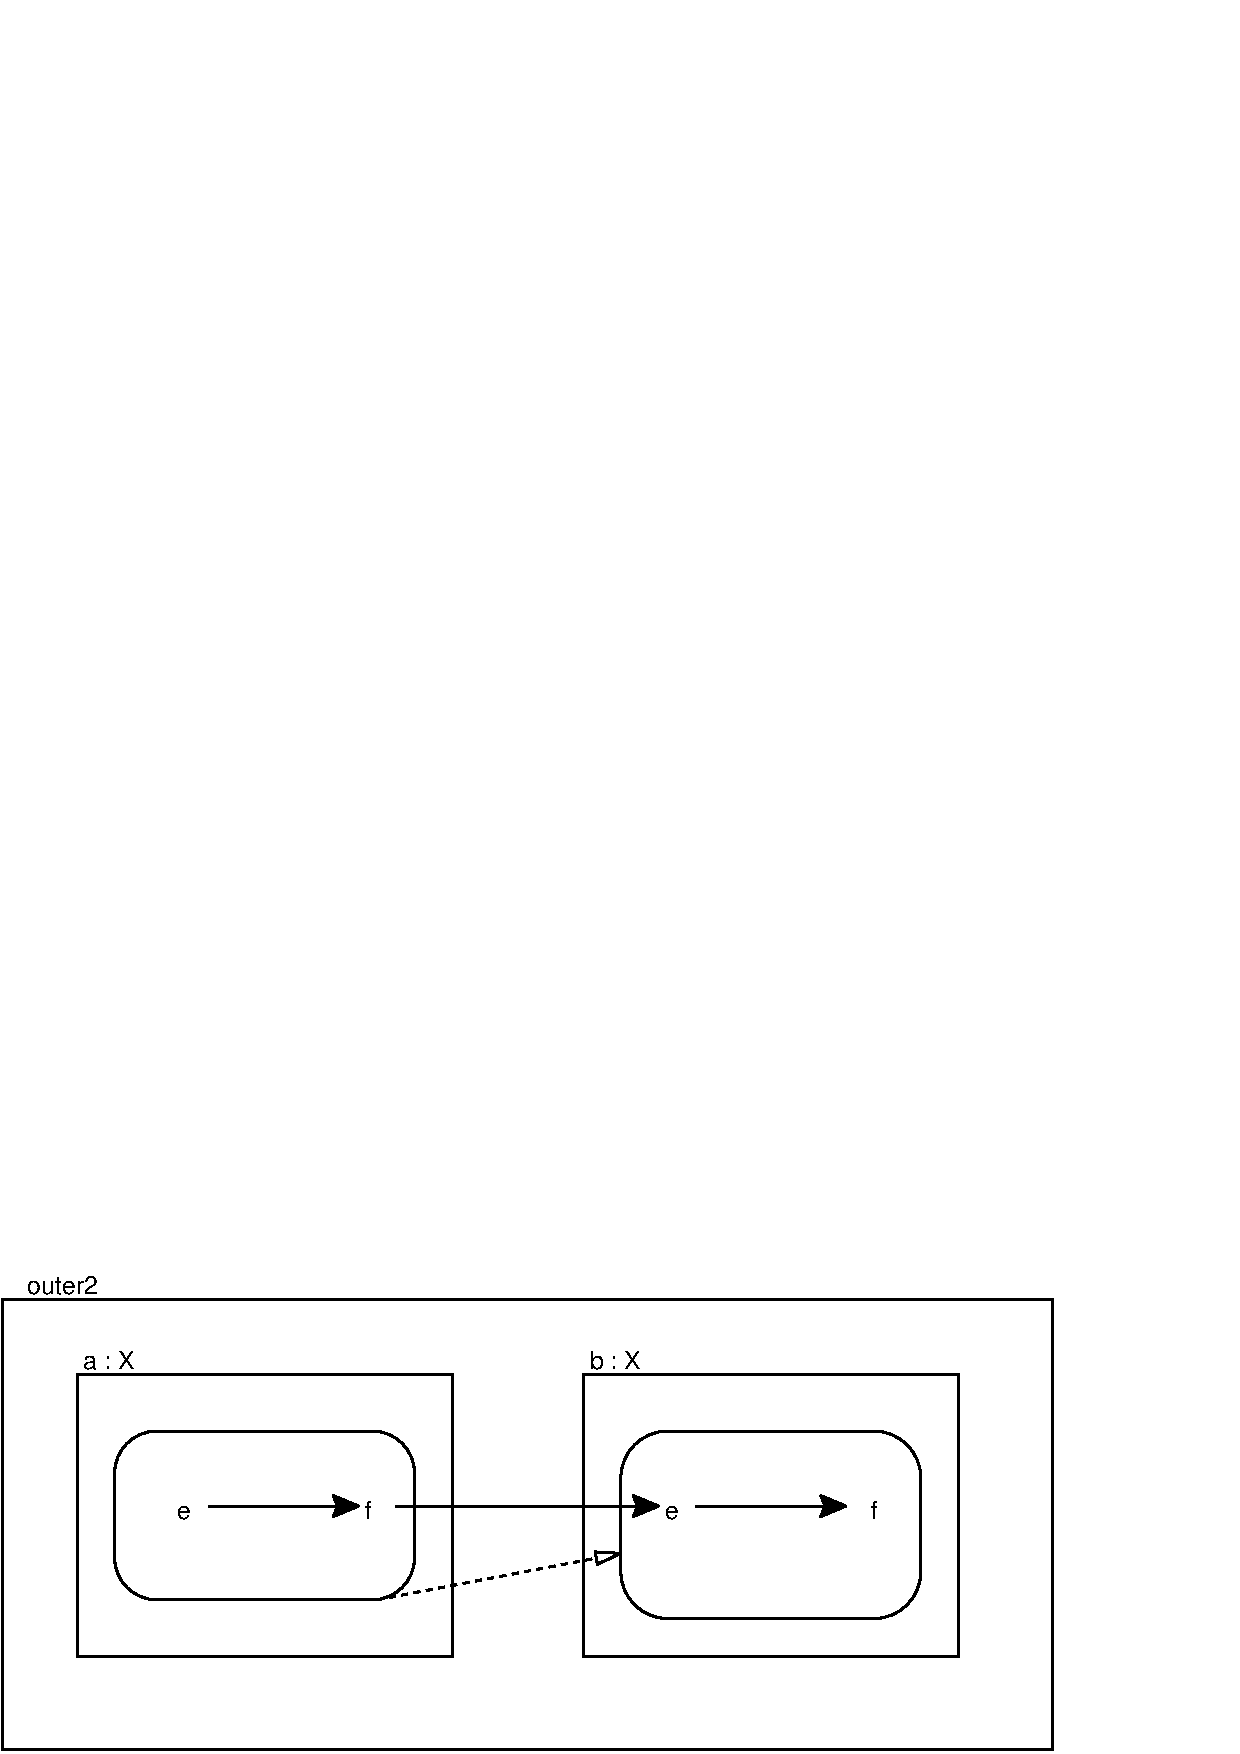
\includegraphics[scale = 0.7]{egdirectlinks}
  \caption{The structure of the \texttt{outer2} model}.
  \label{fig:egdirectlinks}
\end{figure}

\pagebreak

\begin{example}
<?xml version="1.0"?>
<sbml xmlns="http://www.sbml.org/sbml/level3" version="1" level="3">
    <model id="outer2">
        <listOfReactions>
            <reaction id="reaction_1" reversible="false">
                <listOfReactants>
                    <speciesReference stoichiometry="1">
                        <speciesLink object="a">
                            <subobject object="f"/>
                        </speciesLink>
                    </speciesReference>
                </listOfReactants>
                <listOfProducts>
                    <speciesReference stoichiometry="1">
                        <speciesLink object="b">
                            <subobject object="e"/>
                        </speciesLink>
                    </speciesReference>
                </listOfProducts>
                <kineticLaw>
                    <math 
                        <apply>
                            <times/>
                            <cn>0.1</cn>
                            <apply>
                                <csymbol
                                    encoding="SBML" 
                                    definitionURL=
                                        "http://www.sbml.org/symbols/instanceselector">
                                    .
                                </csymbol>
                                <ci>a</ci>
                                <ci>f</ci>
                            </apply>
                        </apply>    
                    </math>
                </kienticLaw>
            </reaction>
        </listOfReactions>
        <listOfSubmodels>
            <model id="X">
                <listOfCompartments>
                    <compartment id="compartmentOne" volume="1"/>
                </listOfCompartments>
                <listOfSpecies>
                    <species id="e" initialAmount="0" compartment="compartmentOne">
                    <species id="f" initialAmount="0" compartment="compartmentOne">
                </listOfSpecies>
                <listOfReactions>
                    <reaction id="reaction_1" reversible="false">
                        <listOfReactants>
                            <speciesReference species="e" stoichiometry="1"/>
                        </listOfReactants>
                        <listOfProducts>
                            <speciesReference species="f" stoichiometry="1"/>
                        </listOfProducts>
                    </reaction>
                </listOfReactions>
            </model>
        </listOfSubModels>
        <listOfInstances>
            <instance
                id="a" 
                xlink:type="simple"
                xlink:href="#xpointer(/sbml/model/listOfSubmodels/model[@id=\%22X\%22])"/>
            <instance
                id="b" 
                xlink:type="simple"
                xlink:href="#xpointer(/sbml/model/listOfSubmodels/model[@id=\%22X\%22])"/>
        </listOfInstances>
        <listOfLinks>
            <link>
                <from object="a">
                    <subobject object="compartmentOne"/>
                </from>
                <to object="b">
                    <subobject object="compartmentOne"/>
                </to>
            </link>
        </listOfLinks>
    </model>
</sbml>
\end{example}

Figure~\ref{fig:egdirectlinks-implied} shows the model implied by \texttt{outer2}.
\begin{figure}[h]
  \vspace*{8pt}
  \centering
  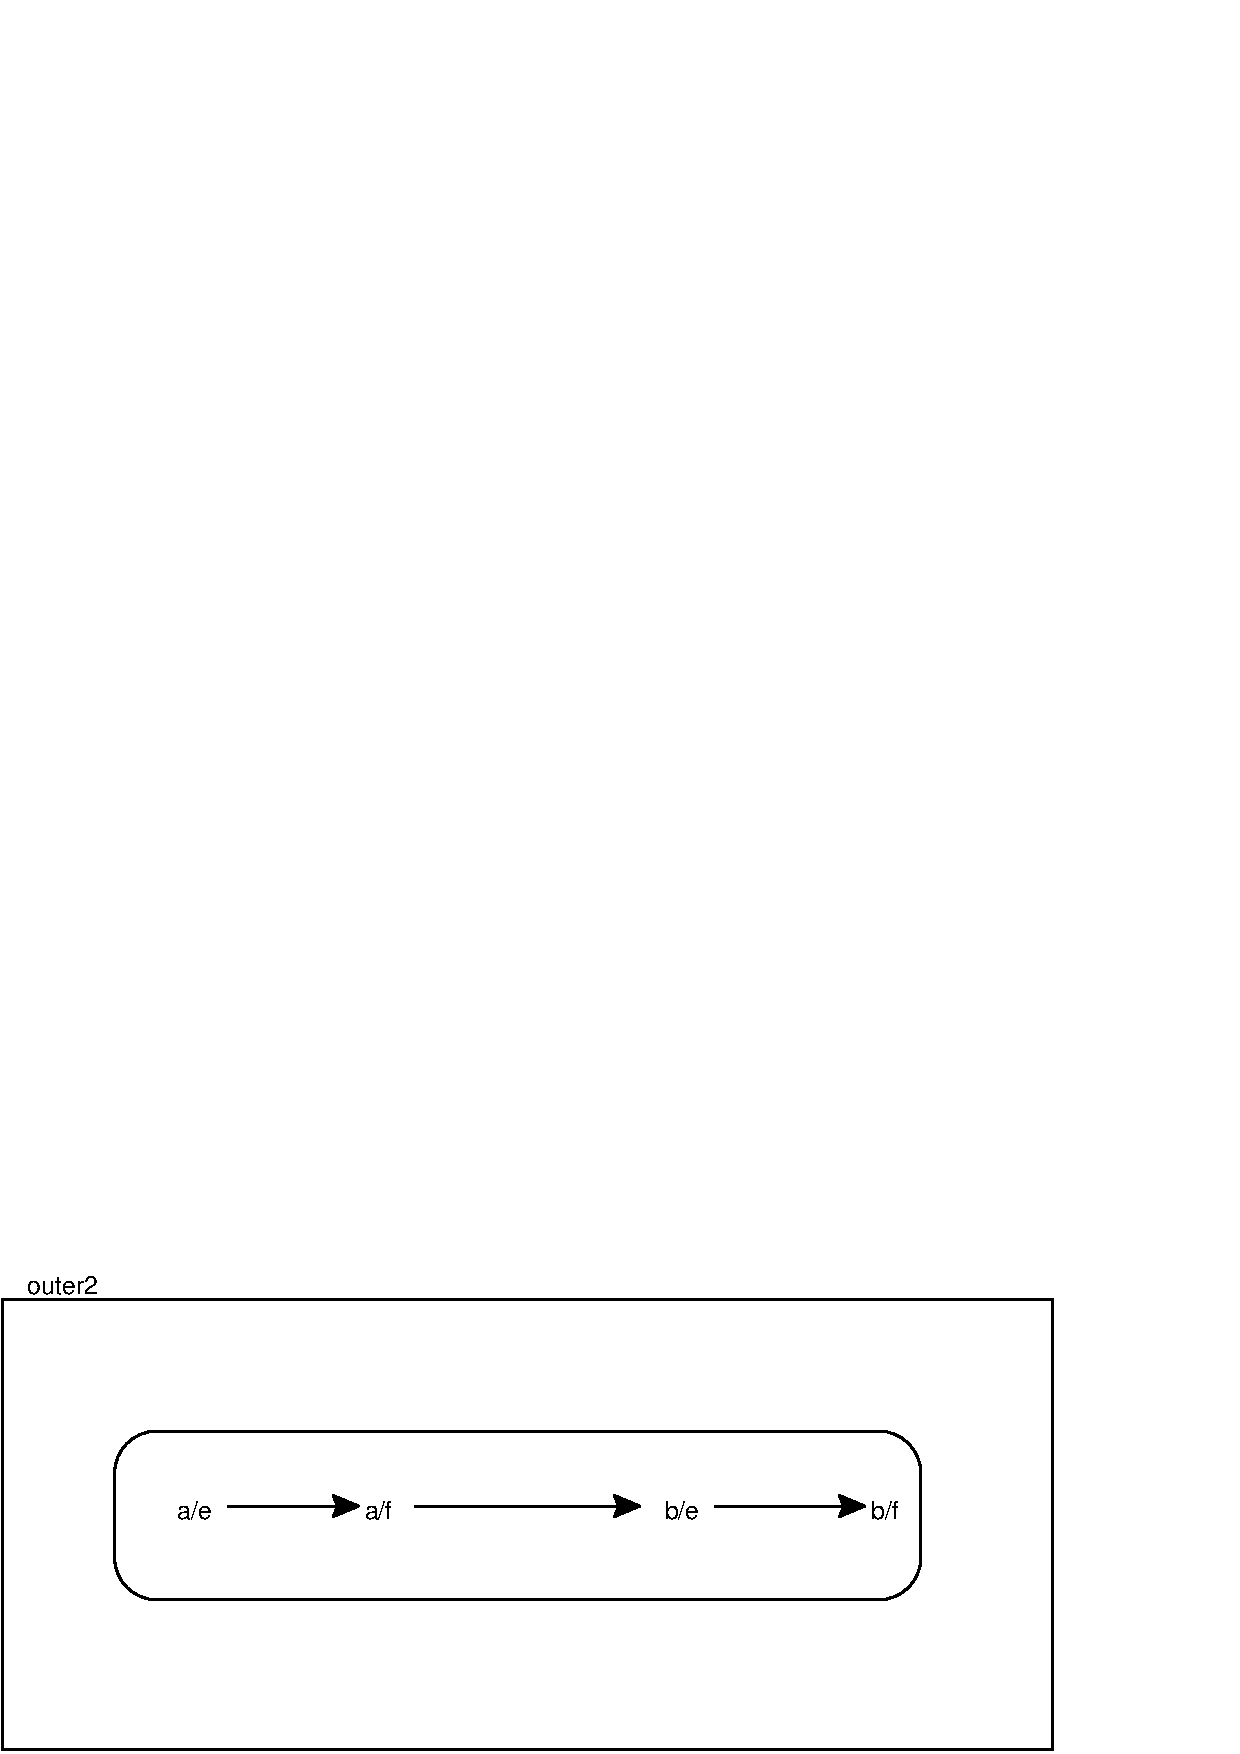
\includegraphics[scale = 0.7]{egdirectlinks-implied}
  \caption{The structure implied by the \texttt{outer2} model}.
  \label{fig:egdirectlinks-implied}
\end{figure}

The array proposal contains a more extensive model that combines
array and model composition features.

%=============================================================================
% References
%=============================================================================

\bibliographystyle{apalike}
\bibliography{strings,a,b,c,d,e,f,g,h,i,j,k,l,m,n,o,p,q,r,s,t,u,v,w,x,y,z}
\end{document}
